\documentclass[a4paper,times,hidelinks,12pt]{article}
\usepackage[top=2.5 cm, bottom=2.5 cm, left=4 cm, right=2.5 cm]{geometry}
\usepackage{amsmath}
\usepackage{multirow}
\usepackage{graphicx}
\usepackage{float}
\usepackage{setspace}
\usepackage[bottom]{footmisc}
%\usepackage{svg}
\usepackage{subcaption}
%\usepackage{minted}
\usepackage{indentfirst}
\usepackage{hyperref}
\usepackage{algorithm}
\usepackage{rotating}
\usepackage[noend]{algpseudocode}

%\makeatletter
%\def\BState{\State\hskip-\ALG@thistlm}
%\makeatother

\newcommand\tab[1][0.5cm]{\hspace*{#1}}
\newcommand*\dif{\mathop{}\!\mathrm{d}}

%\setlength\parindent{0pt}

\begin{document}
%\linespread{1.5}
\onehalfspacing

\begin{titlepage}
\begin{center}
\vspace*{1cm}
\underline{\textbf{\Large ISTANBUL TECHNICAL UNIVERSITY}} \\[10 pt]

\underline{\textbf{\large FACULTY OF SCIENCE AND LETTERS}} \\[15 pt]

\textbf{\large Graduation Project} \\
\vspace{1.8 cm}

\includegraphics[scale=1.2]{itu_logo.pdf} \\
\vspace{1.8 cm}
%\textbf{\large Machine Learning and Nonlinear Schr{\"o}dinger Equation} \\[5 pt]
\textbf{\large Machine Learning and Non-linear Schr{\"o}dinger Equation} \\[5 pt]
\textbf{H{\"u}seyin Talha \c{S}enya\c{s}a}\\
\vspace{1.5 cm}
\end{center}
\vfill
\textbf{{Department : Physics Engineering}}\\
    \textbf{Student ID \hspace{0.2 cm}: 090120132}\\
    \textbf{Advisor\hspace{1.1 cm}: Assoc. Prof. A. Levent Suba\c{s}{\i}}
\vspace{2 cm}

\center\textbf{SPRING 2018}

\end{titlepage}


%\title{\textbf{TEST}}
%\date{}
%\maketitle
\setcounter{page}{1}
\pagenumbering{roman}

\addcontentsline{toc}{section}{Summary}
\section*{Summary}

We train an artificial neural network to estimate the ground state energy
of a one-dimensional Bose-Einstein condensate in different type of potentials including random.
Such a system can be described by the solution of a non-linear Schr{\"o}dinger equation also called a Gross-Pitaevskii equation. We also use the method for the inverse problem of predicting the non-linearity parameter using the ground
state density profile for a given harmonic trapping potential.
\vspace*{\fill}


\newpage

%\section*{\centering ACKNOWLEDGEMENT}
\addcontentsline{toc}{section}{ACKNOWLEDGEMENT}
\begin{center}
\vspace*{4 cm}
\textbf{ACKNOWLEDGEMENT} \\[10 pt]
\end{center}
I would like to express my sincere gratitude to my advisor  Assoc. Prof. A. Levent Suba\c{s}{\i} for the support of this project, for his patience and motivation.\\
\textbf{May, 2018} \hspace{7.75 cm}\textbf{H{\"u}seyin Talha \c{S}enya\c{s}a}


\vspace*{\fill}

\newpage
\tableofcontents

\newpage

\pagenumbering{arabic}
\section{Introduction and Motivation}


\label{sec:Intro}
%\noindent Machine learning.\\
%General usage area.\\
%ML in physics and Phyiscs in ML.\\
%ML\&SE article.\\
%Ours difference.\\



In quantum mechanical systems one must obtain the wave function to determine physical properties of the system. For single particle systems, obtaining the wave function is easy compared to many body systems. The solution can be even harder if the described system involves interactions between particles because such differential equations may have nonlinear terms. In nonlinear case, there are no general rule to solve the equation and they are treated individually in most cases. If there is no analytic solution and approximation is not on the table then the only chance is numerical solution of the equation to obtain the wave function. However, machine learning applications in recent years showed that physical properties of the system can be predicted without solving these equations. \\

The reason why machine learning has such a capability is that artificial neural networks used in machine learning can approximate any continuous function within desired accuracy. This means that if we take $\epsilon > 0$ as desired accuracy,  $\boldsymbol{y} = \boldsymbol{f}(\boldsymbol{x})$ (bold means vector) output of the network and $\boldsymbol{g}(\boldsymbol{x})$ real value of the function, then it is guaranteed that there exists a network that satisfies the relation $||\boldsymbol{g}(\boldsymbol{x}) - \boldsymbol{f}(\boldsymbol{x})|| < \epsilon $. From this point of view, a process or calculation that can be thought of as a function can be represented by a corresponding neural network that mimics this function in desired accuracy \cite{nielsen2015neural}. With this in mind, neural networks have the potential to learn general functions and be exploited for their advantages. Approximate value of the quantity can be determined for different scenarios. \\

Many different kind of applications of machine learning have already been implemented in physics\footnote{For a detailed list, see \cite{physicsml}}. For example, In \cite{carleo2017solving, cai2017approximating} machine learning is applied to quantum many body problems. A machine learning method called Unsupervised Learning to detect patterns in big datasets is used for discovering phase transitions \cite{wang2016discovering}. There are also developed techniques in machine learning inspired from physics such as quantum tensor networks \cite{stoudenmire2016supervised}. Relation between physics and machine learning also caused foundation of a new branch called Quantum Machine Learning which aims to implement a quantum software to make machine learning faster than its classical version \cite{biamonte1611quantum}. \\

In \cite{mills2017deep}, machine learning approach is applied to a 2D Schr{\"o}dinger equation. The authors built a convolutional deep neural network, and trained it to predict ground state energy of the system under four different confining potentials including random potential. Their study showed that machine learning is a promising alternative in electronic structure calculations of quantum systems. In our study inspired from the article mentioned above, we apply machine learning method to the nonlinear Schr{\"o}dinger equation also known as Gross-Pitaevskii equation to predict ground state energy of a Bose-Einstein condensate with random interaction parameter at absolute zero temperature under six different one dimensional trapping potentials including random. 


\section{Gross-Pitaevskii Equation}

A Bose-Einstein Condensate (BEC) at zero temperature is described by Gross Pitaevskii equation (GPE) also known as non-linear Schrodinger Equation (NLSE). It is mean field approximation of a quantum many body system which the hamiltonian of the system is given by;

\begin{equation}
\label{eq:GPE_hamiltonian}
\hat{H} = \sum_{i = 1}^{N} \left(\frac{\boldsymbol{p}_i^2}{2m} + V(\boldsymbol{r}_i) \right) + \frac{1}{2} \sum_{i = 1}^{N} \sum_{j \neq i}^{N} U(|\boldsymbol{r}_i - \boldsymbol{r}_j|)
\end{equation}

\noindent where $\boldsymbol{p}_i$ $i^{th}$ atom's momentum, $\boldsymbol{r}$ is position vector, $m$ is mass, $V$ is external potential and $U$ is interaction between $i^{th}$ and $j^{th}$  atoms. Since the ground state energy is the only possible minimum energy, one can minimize this hamiltonian in order to obtain ground state energy. To do that, the mean field approximation is utilized to represent all bosons with the same wave function since the condensate is at zero temperature which allows to assume that all bosons are at the ground state \cite{pethick2002bose}. The constraint in the minimization step involves satisfying the normalization condition that is given as,


\begin{equation}
\label{eq:GPE_normalization}
\int |\psi(\boldsymbol{r})|^2 \dif^3 \boldsymbol{r} = N    
\end{equation}

\noindent where $N$ is the number of particles in the system. This condition equals to minimizing the thermodynamic potential, free energy $F = E - \mu N$ such that $\delta F = 0 = \delta E - \mu \delta N = 0$ where $\mu$ is chemical potential \cite{pethick2002bose}. If we plug in the corresponding equations to this expression it becomes,  

\begin{equation}
\label{eq:GPE_derivation_free_energy}
F(\psi) = \int \psi^{*}\hat{H}\psi \dif^3\boldsymbol{r} - \mu \int |\psi|^2 \dif^3\boldsymbol{r}
\end{equation}

\noindent Therefore, the problem can be stated as minimization of the above equation \cite{rogel2013gross}. Applying variation method to this equation while treating $\psi^{*}$
and $\psi$ as independent objects and using $U(|\boldsymbol{r}_i - \boldsymbol{r}_j|) = g\delta(\boldsymbol{r}_i - \boldsymbol{r}_j)$ one can obtain Gross Pitaevskii Equation in stationary form as, 

\begin{equation}
\label{eq:GPE_time_indep}
\frac{-\hbar^2}{2m}\nabla^2\psi + V(\boldsymbol{r})\psi + g|\psi|^2\psi = \mu\psi
\end{equation}

%General form of GPE in three dimension is given as,
%
%\begin{equation}
%\label{eq:GPE_3D}
%i \hbar \frac {\partial \psi}{\partial t} = \frac {-\hbar^2}{2m}\nabla^2
%\psi + V(\boldsymbol{r}, t)\psi + g|\psi|^2\ \psi
%\end{equation}

\noindent where $\hbar$ is Planck constant, $\psi(\boldsymbol{r})$ is the wave function, $\nabla^2$ is the Laplacian operator, $g$ is interaction parameter and it is defined as 

\begin{equation}
\label{eq:GPE_inter_param}
g=\frac{4\pi\hbar^2a_s}{m}
\end{equation}

\noindent where, $a_s$ is the s wave scattering length. Nonlinearity of the equation is caused by the cubic term $g|\psi|^2$ which represents the interactions between bosons. The $|\psi|^2$ term is interpreted as density, thus; there occurs an energy contribution caused by the mean field interactions. If there is no interaction GPE reduces to the Schr{\"o}dinger Equation (SE) and becomes a linear equation. By definition, $g$ can be positive or negative. If $g > 0$, it represents repulsive interaction, and if $g < 0$, it represents attractive interactions \cite{pitaevskii2016bose}.

\graphicspath{{"../figs/potentials/"}}
\begin{figure}[H]
    \centering
    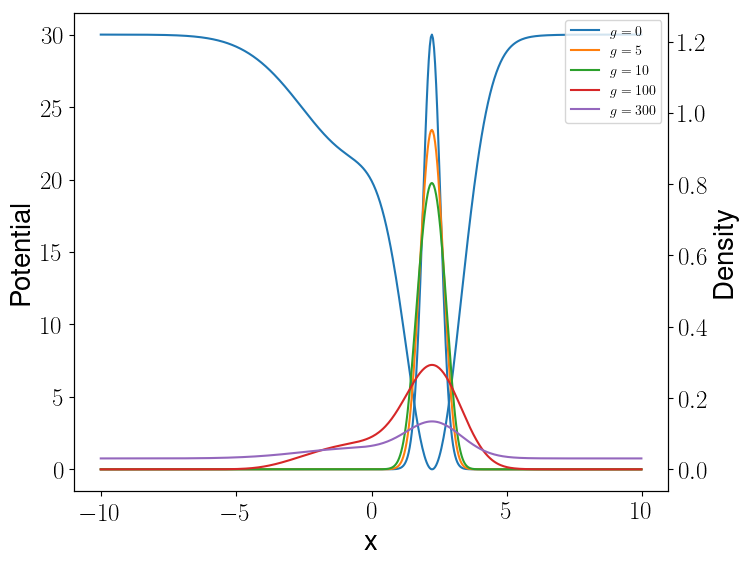
\includegraphics[width=0.6\linewidth]{solutionswithinter}
    \caption{Density under one dimensional double inverted gaussian potential with different interaction parameters. Here density becomes more flatten as the interaction parameter increases.}
\label{fig:gaussian_pot_and_density}
\end{figure}


\noindent The time evolution of the system must occur according to the Schr{\"o}dinger Equation, therefore; the time dependent GPE can be written as,

\begin{equation}
\label{eq:GPE_time_evolution}
i \hbar \frac{\partial\Psi(\boldsymbol{r}, t)}{\partial t} = \hat{H}\Psi(\boldsymbol{r}, t)
\end{equation}

\noindent  where $t$ is time and $\Psi(\boldsymbol{r}, t) = \psi(\boldsymbol{r})e^{-i\mu t/\hbar} $. If it is rewritten in open form,

\begin{equation}
\label{eq:GPE_time_indep}
i \hbar \frac{\partial\Psi(\boldsymbol{r}, t)}{\partial t} = \left[\frac{-\hbar^2}{2m}\nabla^2 + V(\boldsymbol{r}) + g|\Psi(\boldsymbol{r}, t)|^2 \right] \Psi(\boldsymbol{r}, t)
\end{equation}

\noindent The ground state energy of the system is given in Eq.~\eqref{eq:GPE_derivation_free_energy} which is,

\begin{equation}
\label{GPE_total_energy_general}
\langle E \rangle = \int \Psi^{*}\hat{H}\Psi \dif^3\boldsymbol{r}
\end{equation}

\begin{equation}
\label{GPE_total_energy}
E = \int \left(\frac {\hbar^2}{2m}|\nabla
\Psi|^2 + V|\Psi|^2 + \frac{g}{2}|\Psi|^4 \right) \dif^3 \boldsymbol{r}
\end{equation}

\noindent Here, the terms represent kinetic, potential and interaction energy respectively.\footnote{Contribution from the interaction energy is divided by two to eliminate double counting while pairing bosons.} Direct relation between chemical potential and energy can be obtain from integration of the Eq~\eqref{eq:GPE_time_indep}, 

\begin{equation}
\label{eq:mu_and_total_en}
\mu = \frac{E_{kin} + E_{pot} + 2E_{int}}{N}
\end{equation}

\noindent In the non-interacting case this expression leads to energy per particle and if the potential does not depend on time the total energy of the system is conversed. 

 
%\subsection{General information about GPE}
%\subsection{Why and how nonlinearty is introduced.}
%\subsection{Physical and mathematical interpretation of interaction parameter. (phy: attractive, %repulsive  math:dominance of the terms)}
%\subsection{Stationary form.}
%\subsection{Potential, kinetic and interaction energy expressions.}
\subsection{Reduction of Dimension}

Since we are going to work in one dimension, we must express 1D GPE by reducing the dimensionality of the 3D GPE. This reduction of dimension step is done under anisotropic harmonic trapping potential given by;

\begin{equation}
\label{eq:GPE_harmonic_potential}
V(x, y, z) = \frac{1}{2}m(\omega_x^2 x^2 + \omega_y^2y^2 + \omega_z^2z^2)
\end{equation}


\noindent where $\omega_x$,$\omega_y$,$\omega_z$ are angular frequencies. The confinement of the physical dynamics of the system can be performed by making angular frequencies asymmetric such that $\omega_z, \omega_y \gg \omega_x$ and keeping their energy order much greater than condensate's energy $ \hbar(\omega_z \omega_y)^{1/2} \gg \mu $. Now the dynamics of the system only develop in one dimension and it can be described with a corresponding one dimensional GPE equation \cite{barenghi2016primer}. To obtain one dimensional GPE one can rewrite wave function,

\begin{equation}
\label{eq:GPE_time_indep_wave_func_seperated}
\psi(x, y, z, t) = \psi_x(x, t)\psi_y(y)\psi_z(z)
\end{equation}

\noindent $\psi_y$ and $\psi_z$ are the ground state solution of the transverse potentials;

\begin{equation}
\begin{split}
\label{eq:GPE_x_y_wave}
& \psi_y(y) = \frac{1}{{(\pi l_y^2)}^{1/4}}e^{-y^2/2l_y^2} \\
& \psi_z(z) = \frac{1}{{(\pi l_z^2)}^{1/4}}e^{-z^2/2l_z^2}
\end{split}
\end{equation}

\noindent where $l_y = \sqrt{\hbar/m\omega_y}$ and $l_z = \sqrt{\hbar/m\omega_z}$ are the harmonic oscillator lengths that related to the density distribution of the condensate. Normalization of the wave function is chosen such that $\int \psi_y(y) \dif y = \int \psi_z(z) \dif z = 1$, and $\int \psi_x(x, t) = N$. If we plug in the factorized wave function to Eq.~\eqref{eq:GPE_time_indep}, then, the equation becomes;

\begin{equation}
\label{eq:GPE_1D_harmonic}
\mu^{\prime}\psi_x = \frac{-\hbar^2}{2m}\frac{\dif^2\psi_x}{\dif x^2} + \frac{1}{2}m\omega_x^2 x^2\psi_x + g^{\prime}|\psi_x|^2\psi_x 
\end{equation}

\noindent where $\mu^{\prime}$ and $g^{\prime}$ one dimensional effective chemical potential and interaction strength respectively

\begin{equation}
\label{eq:GPE_1D_chem_inter}
\mu^{\prime} = \mu - \frac{\hbar}{2}(\omega_y - \omega_z), \quad g^{\prime} = \frac{g}{2\pi l_y l_z}
\end{equation}

\noindent Here we showed that how interaction parameter and chemical potential are effected when dimension of the 3D GPE is reduced. We are going to use these effective quantities in our study. We also directly used the harmonic potential for simplicity but Eq~\eqref{eq:GPE_harmonic_potential} can be replaced by another equation such as,

\begin{equation}
\label{eq:GPE_harmonic_potential_plus_pot}
V(x, y, z) = V(x) + \frac{1}{2}m(\omega_x^2 x^2 + \omega_y^2y^2 + \omega_z^2z^2)
\end{equation}

\noindent where $V(z)$ can be optical potential for instance \cite{zheng2013dynamics}. Since relation between potential and dimension reduction is not in our scope, we directly change the potential expression with a generic one and accept the one dimensional GPE as,

\begin{equation}
    \label{eq:GPE_1D}
    \frac{-\hbar^2}{2m}\frac{\dif^2\psi_x}{\dif x^2} + V(x)\psi + g|\psi|^2\psi = \mu\psi
\end{equation}

\noindent and from now on, we refer to Eq.~\eqref{eq:GPE_1D} as GPE.

\subsection{Analytic Solution and Thomas-Fermi Approximation}

There is no general solution of GPE. Known analytic solutions exist only for few cases and lack of analytic solution is also one of the main motivation of the application of machine learning technique. In our study, infinite well and harmonic potential with zero interaction parameter has analytic solutions. Here we give the ground state wave solution and energy of the harmonic potential in non-interacting case which is also solution of the SE,

\begin{equation}
\label{eq:harmonic_ground_state_wave}
    \psi(x) = (\frac{m\omega}{\pi\hbar})^{1/4}\exp^{-m\omega x^2/\hbar}
\end{equation}

\begin{equation}
\label{eq:GPE_1D_solution_harmonic}
    E = \mu = \frac{1}{2}\hbar\omega
\end{equation}

\noindent respectively. Comparison of the numerical solution and analytic solution in given in the figure.

\graphicspath{{"../figs/numericanalyze/"}}
\begin{figure}[H]
\centering
    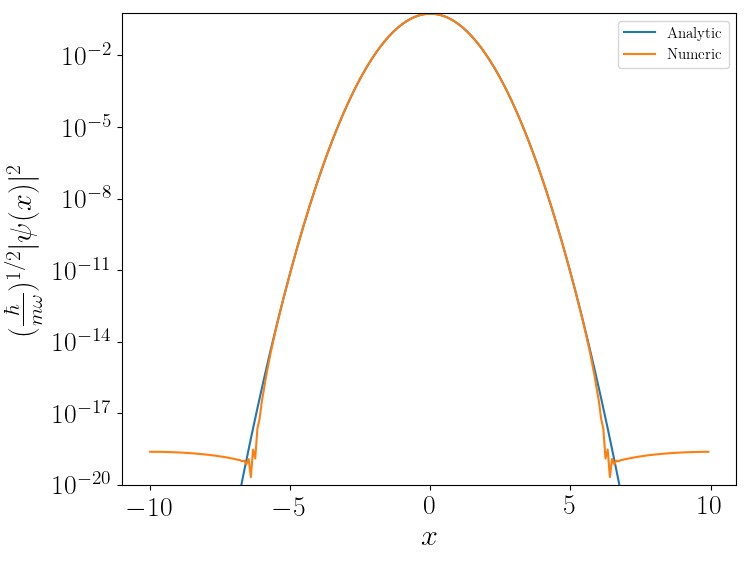
\includegraphics[width=0.6\linewidth]{sol-comp}
\caption{Here we give comparison of known analytic solution and corresponding numerical solution in log scale. As it is shown that the numerical solution framework able to produce solution with high precision. The wave function goes to zero at numerical infinity as in the analytic solution.}
\label{fig:dens_energy_error}
\end{figure}


GPE generally solved by numerically or by approximation such as variational calculation or Thomas-Fermi approximation. In the following section we briefly introduce Thomas-Fermi approximation and then we add comparison with numerical solutions. \\

\textbf{Thomas Fermi Approximation}\\


It is said that the second derivative term with respect to position represents the kinetic energy. When the potential and the interaction energy are dominant compared to the kinetic energy, the kinetic term can be neglected. This situation occurs when the condensate is large adequately and the interaction between bosons is repulsive \cite{pethick2002bose}. In another perspective, neglecting the kinetic term equivalent to making an assumption that there is no difference between the energy requirements to add a particle at arbitrary points \cite{rogel2013gross}. When the kinetic term is dropped, the new equation can be written as;

\begin{equation}
\label{eq:GPE_1D_thomas_fermi}
    V(x)\psi(x) + g|\psi(x)|^2\psi(x) = \mu\psi(x)
\end{equation}
\noindent this equation is analytically solvable and the solution is given by,


\begin{equation}
\label{eq:thomas_fermi_solution}    
n(x) = |\psi(x)|^2 =  
    \begin{cases}
        (\mu_{TF} - V)/g &\quad\text{if }  |x| \le x_{TF}  \\
        0 &\quad \textit{otherwise} \\
    \end{cases}
\end{equation}

\noindent where $x_{TF}$ is called Thomas-Fermi Length and $n(x)$ is density. The density defined in this range and cannot be negative, therefore; if the normalization condition Eq.~\eqref{eq:GPE_normalization} is applied then the equation reads,  

\begin{equation}
    \label{eq:thomas_fermi_mu_integral}
        \int_{-\infty}^{\infty} |\psi|^2 \dif x = \int_{-x_{TF}}^{x_{TF}} \frac{(\mu - V)}{g} \dif x = N 
    \end{equation}

\noindent With this equation, density of the system can be obtain via invoking boundary conditions. For an exact analytic expression example, one dimensional harmonic potential can be used, 

\begin{equation}
   \frac{1}{g} \left [ \int_{-x_{TF}}^{x_{TF}} \mu \dif x - \int_{-x_{TF}}^{x_{TF}} \frac{1}{2}m\omega^2x^2 \dif x \right ] = N
\end{equation}

\begin{equation}
\label{eq:thomas_fermi_integral_result}
    \frac{2\mu x_{TF}}{g} - \frac{m\omega^2 x_{TF}^3}{3g} = N
\end{equation}


\noindent From boundary conditions,
\begin{equation}
\label{eq:thomas_fermi_mu_bound}
    \mu = V(x_{TF}) = \frac{1}{2}m\omega^2x_{TF}^2    
\end{equation}


\noindent If we combine Eq.~\eqref{eq:thomas_fermi_integral_result} and Eq.~\eqref{eq:thomas_fermi_mu_bound} the equations reads,

\begin{equation}
    \frac{m\omega^2 x_{TF}^3}{g} - \frac{m\omega^2 x_{TF}^3}{3g} = N
\end{equation}


\begin{equation}
    \frac{4}{3} \left( \frac{2\mu}{m\omega^2} \right)^{1/2} \frac{\mu}{g} = N
\end{equation}

\begin{equation}
    \mu = \left(\frac{9}{32} (N\omega g)^2 m \right)^{1/3}
\end{equation}

\noindent Here we give comparison of densities obtained by numerical solution and Thomas-Fermi approximation for different potential types. 

\graphicspath{{"../figs/numericanalyze/"}}
\begin{figure}[H]
\centering
\begin{subfigure}[t]{0.45\textwidth}
    \includegraphics[width=\linewidth]{{{thomas-fermi-random-15.0}}}
    \caption{Random Potential Type 1}
    \label{fig:a}
\end{subfigure}
\begin{subfigure}[t]{0.45\textwidth}
    \includegraphics[width=\linewidth]{{{thomas-fermi-random2-15.0}}}
    \caption{Random Potential Type 2}
    \label{fig:b}
\end{subfigure}
\begin{subfigure}[t]{0.45\textwidth}
    \includegraphics[width=\linewidth]{{{thomas-fermi-random3-15.0}}}
    \caption{Random Potential Type 3}
    \label{fig:c}
\end{subfigure}
\begin{subfigure}[t]{0.45\textwidth}
    \includegraphics[width=\linewidth]{{{thomas-fermi-harmonic-15.0}}}
    \caption{Harmonic Potential}
    \label{fig:d}
\end{subfigure}
\caption{Here the potential types are labeled. The interaction parameter $g$ is 15.}
\label{fig:comp_thomas_num}
\end{figure}

As shown in Fig~\ref{fig:comp_thomas_num}d, the interaction parameter is great enough to use Thomas-Fermi approximation but it is known that it starts to fail as $g$ goes to lower values.

\subsection{Numerical Solution and Potential Generation Process}

The dataset -which will be defined in detail later- generation step is divided into two main parts and implemented independently. The first one is generating desired potential and the second one is numerical solution of the GPE under this potential by giving the generated potential to the numerical solution framework. The detailed description of the potential generation process is given in section~\ref{sec:potential_generation}. \\

In numerical solution part, we use a framework called XMDS \cite{dennis2013xmds2}, implemented specifically to solve differential equation systems with well optimized numerical methods. In this framework partial differential equation systems can be described by a markup language called XML.  When equation system is declared properly, XMDS produces a source code written in C++ that solves the equation with specified numerical method. Because of modularity in our implementation, the framework only solves the equation by supplied parameters, the framework does not generate anything internally such as potential, even the scaling factors are supplied externally. Such a modularity has an huge advantage such that changing numerical solution framework does not effect potential generation step, therefore; the work to change numerical solution framework is minimized. The only requirement is implementation of input output operations. By using this advantage, we also use another numerical solution framework called GPELab \cite{antoine2014gpelab} implemented in Matlab to compare solutions' consistency and effect of scaling.


\subsubsection{Scaling}

The scaling of GPE is generally done according to potential type and there are more than one scaling conventions. In this section we use a more general approach to scale GPE since the solutions will be numerical and we briefly would like to investigate how different scalings affect the solutions' consistency. To do that, the dimensionless quantities are introduced with variable coefficients so that scaling coefficient controlled by these variables. 

First we define dimensionless potential, and then we make the length dimensionless,

%\begin{equation}
%%    \label{eq:GPE_1D}
%    \frac{-\hbar^2}{2m}\frac{d^2\psi}{dz^2} + V(x)\psi + g|\psi|^2\psi = \mu\psi
%\end{equation}


$$ \overline{V}(x) \equiv \frac{V(x)}{\gamma E_0}, \qquad \widetilde{x} \equiv \frac{x}{\beta L} $$

\noindent Here $\gamma$ and $\beta$ positive real numbers. $E_0$ is in energy unit and $L$ is in length and they are defined respectively as;

$$E_0 = \frac{\hbar^2}{2m} $$

\noindent The potential can also be transformed in length scale such that; 

$$ \widetilde{V}(\widetilde{x}) \equiv \overline{V}(\beta L x) $$ 

\noindent If these transformations are pluged into the Eq.~\eqref{eq:GPE_1D} it becomes,

\begin{equation}
    \label{eq:GPE_1D_dimensionless_en_len}
    \frac{-\hbar^2}{2m\gamma E_0} \frac{1}{\beta^2 L^2}  \frac{d^2\psi}{d \widetilde{x}^2} + \widetilde{V}(\widetilde{x})\psi + \frac{g}{\gamma E_0}|\psi|^2\psi = \frac{\mu}{\gamma E_0}\psi
\end{equation}

\noindent To obtain final form, we define dimensionless chemical potential, wave function and interaction parameter respectively. 

$$\widetilde{\mu} \equiv \frac{\mu}{\gamma E_0}, \qquad \widetilde{\psi} \equiv \psi{\sqrt{\frac{\beta L}{N}}}, \qquad \widetilde{g} \equiv \frac{gN}{\gamma E_0 \beta L} $$

\noindent To control scaling coefficients we set the coefficient of the kinetic term to an arbitrary positive real number $\alpha$  

$$ \frac{\hbar^2}{2m\gamma E_0} \frac{1}{\beta^2 L^2} = \alpha  , $$

\noindent Now the scaling of GPE can be controlled by $\alpha$ and $\beta$ only.

\begin{equation}
\label{eq:GPE_dimensionless}
    -\alpha\frac{d^2\widetilde{\psi}}{d\widetilde{x}^2} + \widetilde{V}(\widetilde{x})\widetilde{\psi} + \widetilde{g}|\widetilde{\psi}|^2 \widetilde{\psi} = \widetilde{\mu} \widetilde{\psi}
\end{equation}
    
Changing $\beta$ directly effects the length scale and it requires extra transformations in potential generation steps, therefore; we are going to change only $\alpha$ to see the effect of scaling by comparing results. An example of setting the scale coefficients is shown in appendix~\ref{ap:scale}.


\graphicspath{{"../figs/numericanalyze/"}}
\begin{figure}[H]
\centering
    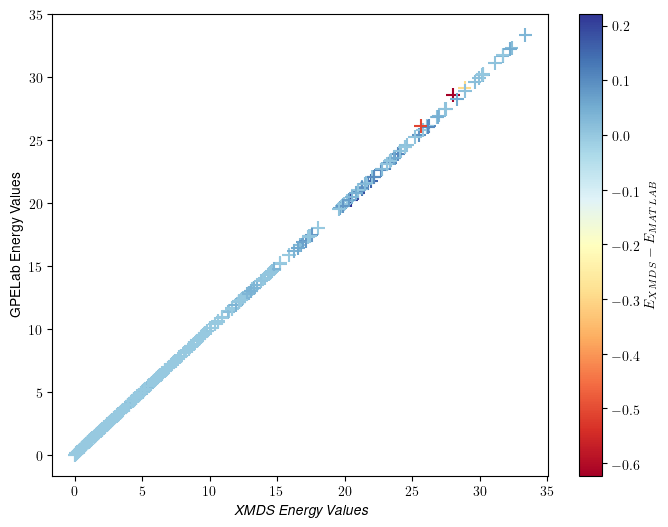
\includegraphics[width=0.6\linewidth]{comparison-energy}
\caption{Energy results comparison of different frameworks, XMDS and GPELab}
\label{fig:dens_energy_error}
\end{figure}


%\subsubsection{Brief info about imaginary time evolution. (detailed in APPENDIX)}
%\subsubsection{XMDS framerwork and other programs.}
\subsubsection{Potential generation} \label{sec:potential_generation}

In potential generation, we built a modular structure such that the algorithms to generate potentials are independent from the restrictions forced by numerical techniques such as boundary conditions or scaling. A python class object responsible for handling this process. This class is constructed with suitable parameters such as "number of points", "width" etc. The generated potentials are sent to another method supplied by class which re-scales, and applies an envelope function to ensure that potential goes to numerical limit at boundaries which is given as,
\begin{equation}
\label{eq:potential_boundary_conditions}
\begin{split}
    V(x < x_l) = V_0 \\ 
    V(x > x_r) = V_0
\end{split}
\end{equation}

To handle these conditions, we define two envelope functions given by the following expressions, 

\begin{equation}
\label{eq:envelope_potential_lr}
    \text{Env}_{LR}(x) = [(1 + \tanh{(\beta(x + x_L))}) + (1 - \tanh{(\beta(x + x_R))})]/2
\end{equation}

\begin{equation}
\label{eq:envelope_potential_m}
    \text{Env}_{M}(x) = 1 - \text{Env}_{LR}(x)
\end{equation}

\noindent where $x_L$ and $x_R$ are bounds given in the Table~\eqref{tb:general_table} and the plot is given in Fig.~\ref{fig:envelope_and_random_withot_pros}.  

\graphicspath{{"../figs/potentials/"}}
\begin{figure}[H]
\centering
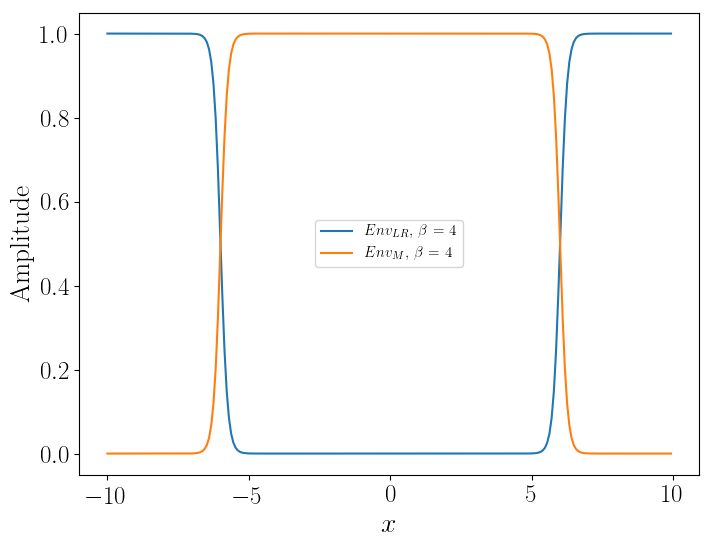
\includegraphics[width=.8\linewidth]{env}
\caption{Envelope Function}
\label{fig:envelope_and_random_withot_pros}
\end{figure}

As shown in Fig.~\ref{fig:envelope_and_random_withot_pros} $Env_{M}$ neutralizes the values while $x$ goes to boundaries and only the region in the middle survives. For $Env_{LR}$ the scenario is vice versa. Simultaneous application of these functions plus re-scaling brings the potential desired form shown in Fig.~\ref{fig:random_plus_envelope}


\graphicspath{{"../figs/potentials/"}}
\begin{figure}[H]
    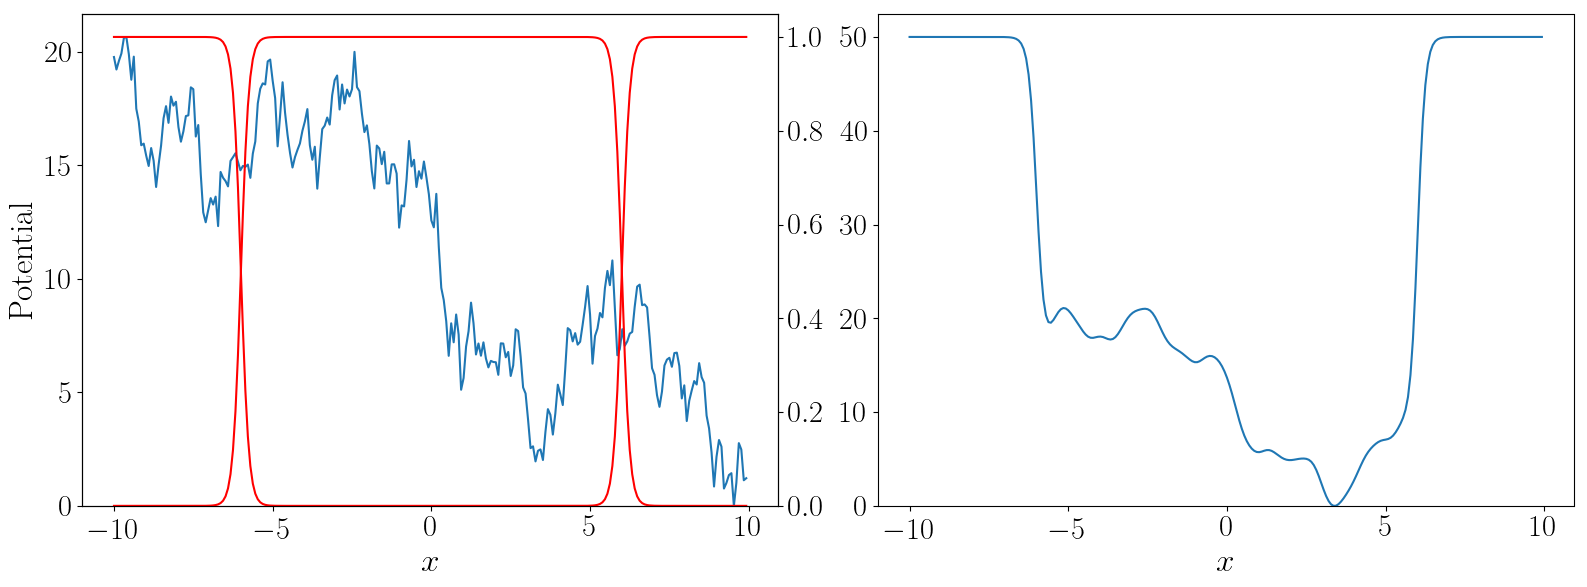
\includegraphics[width=\linewidth]{randombeforeafterproc}
\caption{Envelope functions are applied to a random potential. After that, a gaussian filter is applied for smoothness. We also make sure that the minimum value of the potential is zero at re-scaling process.}
\label{fig:random_plus_envelope}
\end{figure}





\subsubsection{Potential Types}

Bose-Einstein condensates are generally worked with harmonic trapping potential, but we use six different types of potential in our study. The first three potentials are infinite well, harmonic, and double inverted gaussian potential. Their parametric details are given in Table~\ref{tb:general_table}. and the other three are random potentials generated by different algorithms. We investigate training results first individually so that type of the potential in both training and prediction process are same, then we do a cross scenario in that case the type of the potential in training and prediction are different.

\newcommand{\infinitewell}{$
V(x) = 
    \begin{cases}
       0 &\quad\text{if } x_l < x < x_r  \\
       \infty &\quad\text{if } \textit{otherwise} \\
    \end{cases}
$}

\newcommand{\harmonicpot}{$ V(x) =  \frac{1}{2}m \omega^2 (x - x_0) ^2 $}
\newcommand{\gaussianpot}{$V(x) = -A_1 \exp(\frac{(x - \mu_1)^2}{\sigma_1^2}) -A_2 \exp(\frac{(x - \mu_2)^2}{\sigma_2^2})$}
\newcommand{\randomexplation}{Damping high frequencies in Fourier space, and inverse transformation}
\newcommand{\envelopepotLR}{$\text{Env}_{LR}(x) = [(1 + \tanh{(\beta(x + x_L))}) + (1 - \tanh{(\beta(x + x_R))})]/2$}
\newcommand{\envelopepotM}{$\text{Env}_{M}(x) = 1 - \text{Env}_{LR}(x)$}
\newcommand{\randompotONE}{$V(x_{i+1}) = V(x_i) + [X\sim\mathcal{N}(\mu, \sigma)$]}



\begin{sidewaystable}
\begin{table}[H]
\centering
\caption{Potentials}
\label{tb:general_table}
\begin{tabular}{|l|l|l|l|l|l|l|} \hline
Potential                      & Analytic Form / Explanation         & Parameters           & Description       & Min   & Max  \\ \hline
\multirow{3}{*}{Envelope}      & \multirow{2}{*}{\envelopepotLR}     & $x_L$                & Left              & -9    & 4.5  \\ 
                               & \multirow{2}{*}{\envelopepotM}      & $x_R$                & Right             & -4.5  & 9    \\
                               &                                     & $\beta$              & Rapidness         & -4.5  & 9    \\ \hline
\multirow{3}{*}{Infinite Well} & \multirow{3}{*}{\infinitewell}      & $x_l$                & Left Well         & -9    & 4.5  \\ 
                               &                                     & $x_r$                & Right Well        & -4.5  & 9    \\
                               &                                     & $x_r - x_l$          & Width             & 1     & 8    \\ \hline
\multirow{2}{*}{Harmonic}      & \multirow{2}{*}{\harmonicpot}       & $\omega$             & Angular Freq.     & 0.01  & 3    \\ 
                               &                                     & $x_0$                & Equilibrium       & -5    & 5    \\ \hline
\multirow{3}{*}{DI Gaussian}   & \multirow{3}{*}{\gaussianpot}       & $A_1, A_2$           & Amplitude         & 1     & 10   \\ 
                               &                                     & $\mu_1, \mu_2$       & Mean              & -5    & 5    \\
                               &                                     & $\sigma_1, \sigma_2$ & Standard Dev.     & 0.5   & 4    \\ \hline
\multirow{2}{*}{Random\#1}     & \multirow{2}{*}{\randompotONE}      & $\mu$                & Mean              & -4    & 4    \\ 
                               &                                     & $\sigma$             & Standard Dev.     & 0.5   & 4    \\ \hline
Random\#2                      & \randomexplation                    & $k_c$                & Cutoff Wavelength & 1     & 100  \\ \hline
Random\#3                      & Subtraction of two binary grid      & Scale Factor         &                   & 8     & 8    \\ \hline

\end{tabular}
\end{table}
\end{sidewaystable}



\subsubsection{Random Potential Generation}
\label{sec:random_potential_gen}

To be able to observe the effect of random potential generation to the results we use three different random potential generation algorithms. The first one is random walk with random step size such that the first value of the potential array is initialized with a random number. After that, another random number is added to this value to obtain the next element of the array and so on. The distribution of the random numbers is gaussian in this process. The resultant array is not guaranteed to be smooth. Gaussian filter is applied with a random sigma value to the potential array to make it smooth.    

\begin{algorithm}[H]
    \caption{RandomPotential1}\label{euclid}
    \begin{algorithmic}[1]
    \Procedure{RandomPotential1}{}
        \State $ Points = GaussianDistributedRandomPoints()$
        \State $Len = \textit{Length(Points)}$
        \State $Potential[0] = Points[0]$
        \For{$\text{i} = 0 \textbf{ to } Len - 1$}
        \State $Potential[i + 1] = Potential[i] + Points[i]$
        \EndFor
        \State $Potential = GaussianFilter(Potential, \sigma)$ 
    \EndProcedure
    \end{algorithmic}
\label{alg:random_potential_1}
\end{algorithm}

\graphicspath{{"../figs/potentials/"}}
\begin{figure}[H]
    \centering
        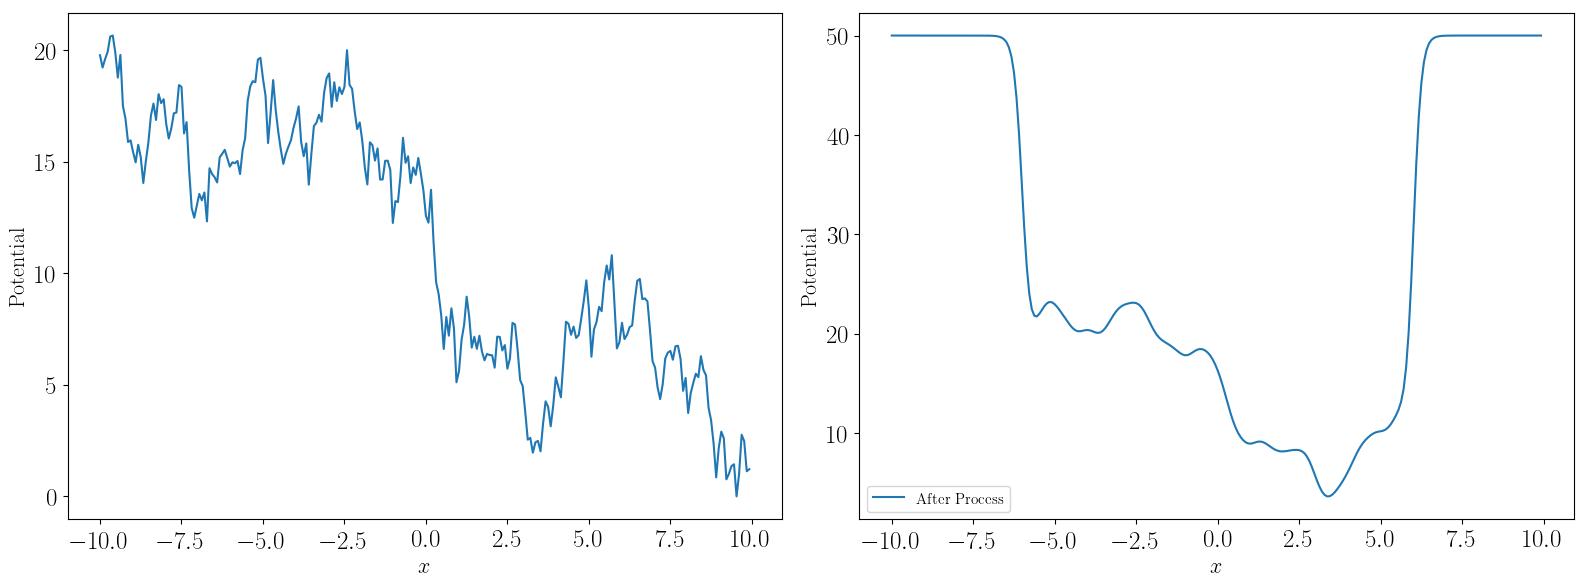
\includegraphics[width=\linewidth]{random-1-noprocandproc}
\caption{Random Potential 1 Before and After Process}
\label{fig:random1_before_after}
\end{figure}

The second algorithm is based on Fourier transformation described in \cite{akkermans2008numerical}. We uniformly select random numbers in real space and apply Fourier transformation to switch Fourier space. After that, an exponential term with great enough coefficient is applied to the high frequencies to absorb them. With this way the smoothness and rapidness of the potential is set without applying gaussian filter.

\begin{algorithm}[H]
    \caption{RandomPotential2}\label{euclid}
    \begin{algorithmic}[1]
    \Procedure{RandomPotential2}{}
        \State $V_i = UniformDistributedNumbers()$
        \State $k = DiscreteFourierTransformSampleFrequencies()$
        \State $k_c = \textit{CutoffWaveLength}$
        \State $V_k = FourierTransform(V_i)$
        \State $V_k = V_k \exp(-k/k_c)^M$
        \State $V_i = InverseFourierTransform(V_k)$
    \EndProcedure
    \end{algorithmic}
\label{alg:random_potential_1}
\end{algorithm}

\graphicspath{{"../figs/potentials/"}}
\begin{figure}[H]
    \centering
        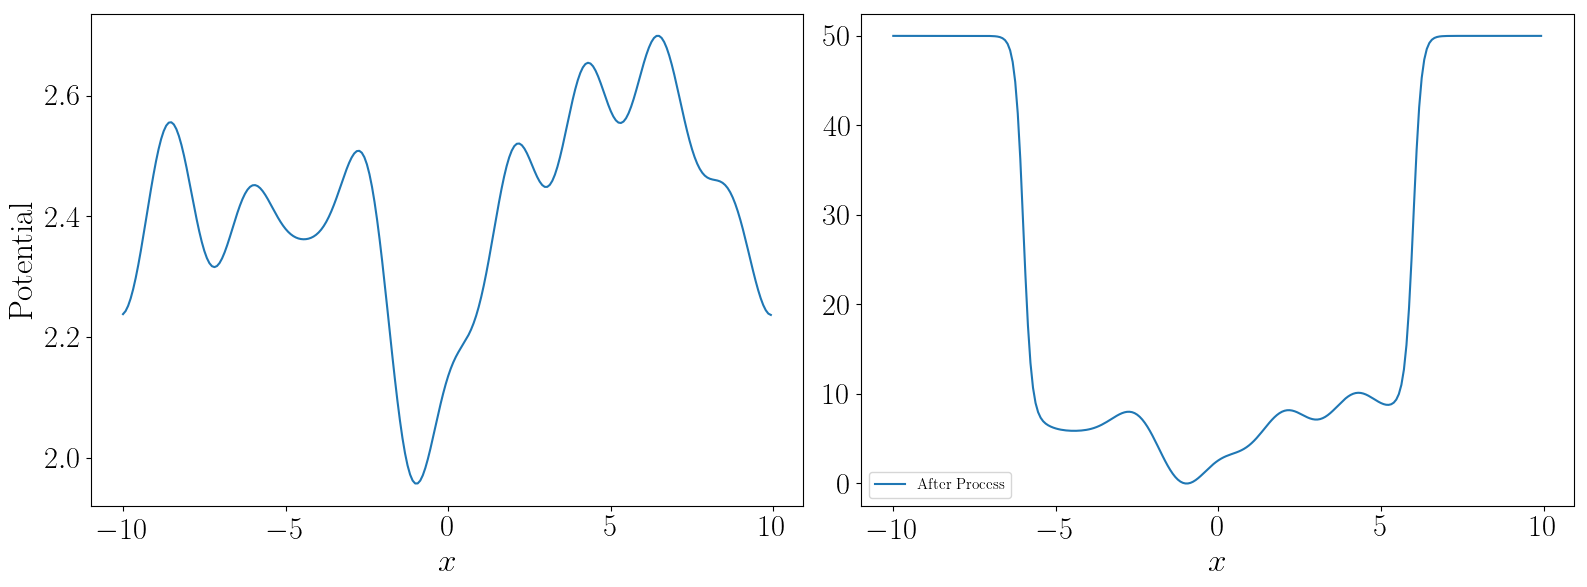
\includegraphics[width=\linewidth]{random-2-noprocandproc}
\caption{Random Potential 2 Before and After Process}
\label{fig:random2_before_after}
\end{figure}

The third one is one dimensional version of the algorithm described in \cite{mills2017deep} with slight modification. First a binary array of length $16$ is generated by assigning random ones or zeros. Then the array is upscaled to $128$ by repeating each element of the array $8$ times. After that, another binary array of length $8$ is generated with the same procedure and upscaled to $64$ by repeating elements. Left and right paddings of length $32$ is added to the second binary array to be able to do element wise substraction between two binary array. Then, the second array is substracted from the first one to obtain the potential in binary form. Finally, a gaussian filter is applied to make the potential smooth. 

\begin{algorithm}[H]
    \caption{RandomPotentia3}\label{euclid}
    \begin{algorithmic}[1]
    \Procedure{RandomPotential3}{}
        \State $ \textit{ScaleFactor} = 8$
        \For{$\text{i} = 0 \textbf{ to } \textit{NumberOfPoints/ScaleFactor}$}
        \State $BinaryGrid[i] = RandomInteger(0, 1)$
        \EndFor
        \State $BinaryGrid = RepeatElements(BinaryGrid, ScaleFactor)$
        \For{$\text{i} = 0 \textbf{ to } NumberOfPoints/(ScaleFactor * 2)$}
        \State $BinaryGrid2[i] = RandomInteger(0, 1)$
        \EndFor
        \State $BinaryGrid2 = RepeatElements(BinaryGrid, ScaleFactor)$
        \State $Padding = Zeros((Length(BinaryGrid) - Length(BinaryGrid2))/2)$
        \State $BinaryGrid2 = Concatanate(Padding, BinaryGrid2, Padding) $
        \State $Potential = BinaryGrid - BinaryGrid2$
        \State $Potential = GaussianFilter(Potential, \sigma)$ 
    \EndProcedure
    \end{algorithmic}
\label{alg:random_potential_1}
\end{algorithm}

\graphicspath{{"../figs/potentials/"}}
\begin{figure}[H]
    \centering
        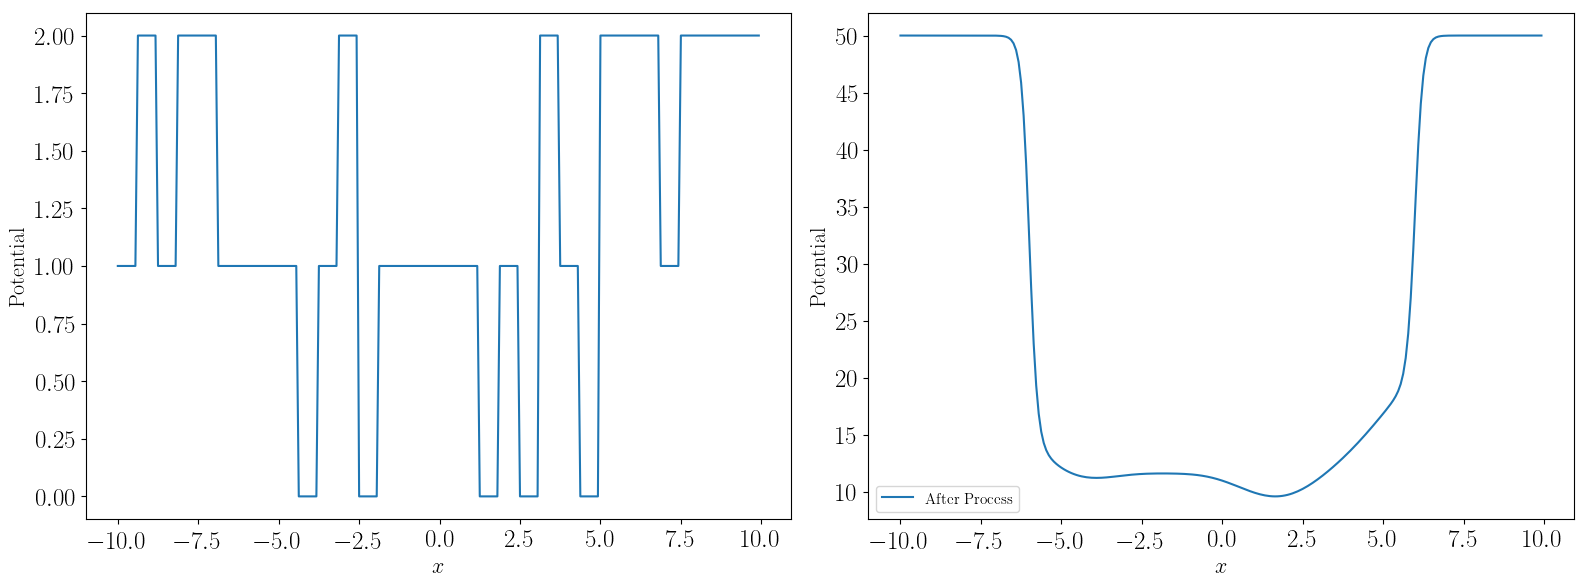
\includegraphics[width=\linewidth]{random-3-noprocandproc}
\caption{Random Potential 3 Before and After Process}
\label{fig:random3_before_after}
\end{figure}

\subsubsection{Density and Ground State Energy}

\graphicspath{{"../figs/potentials/"}}
\begin{figure}[H]
    \centering
    \begin{subfigure}[t]{0.45\textwidth}
        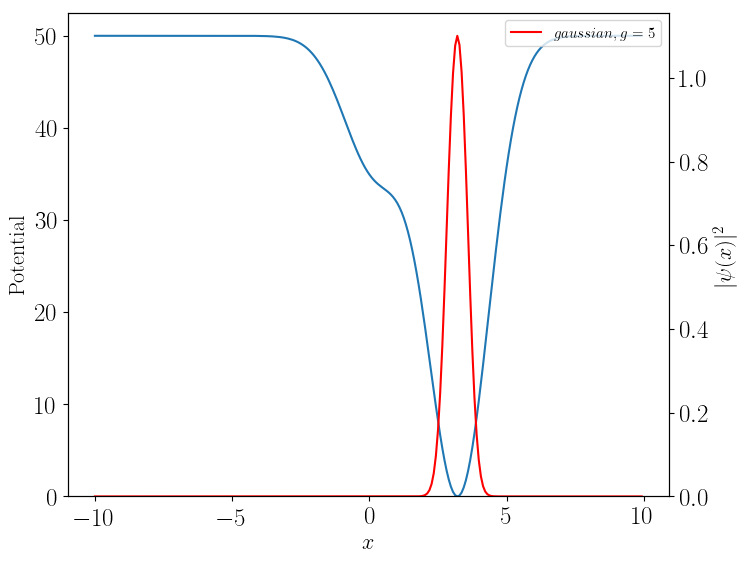
\includegraphics[width=\linewidth]{potvsdensity-gaussian}
    \end{subfigure}
    \begin{subfigure}[t]{0.45\textwidth}
        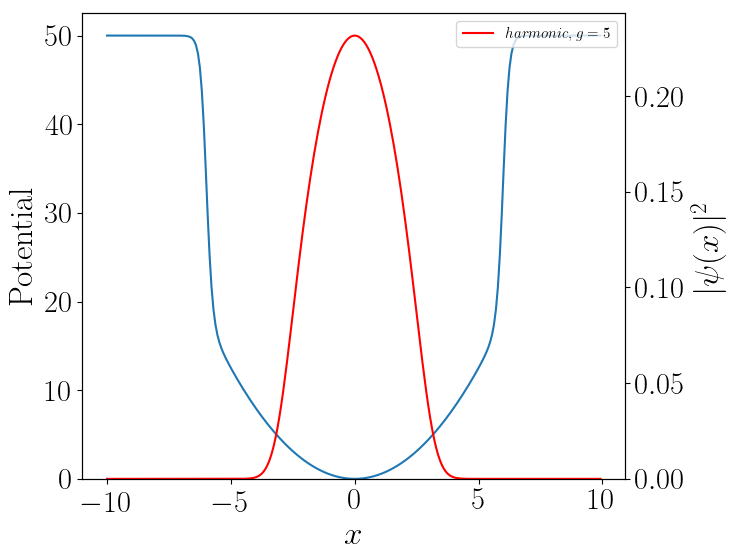
\includegraphics[width=\linewidth]{potvsdensity-harmonic}
    \end{subfigure}
    \begin{subfigure}[t]{0.45\textwidth}
        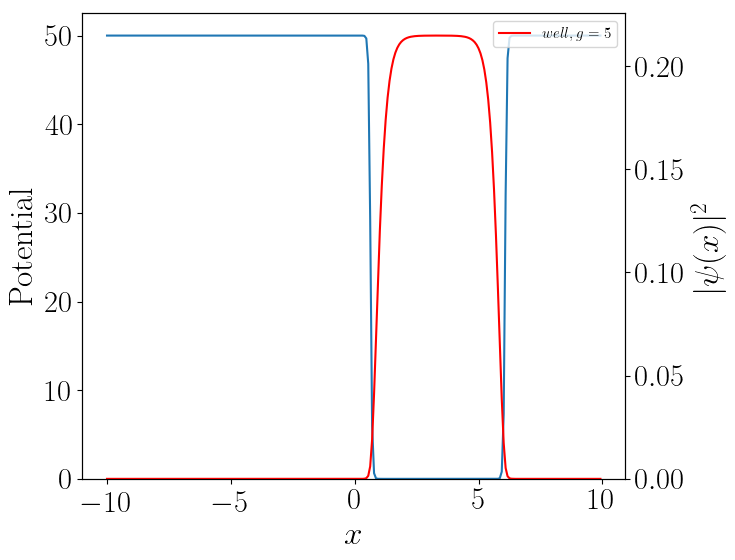
\includegraphics[width=\linewidth]{potvsdensity-well}
    \end{subfigure}
    \begin{subfigure}[t]{0.45\textwidth}
        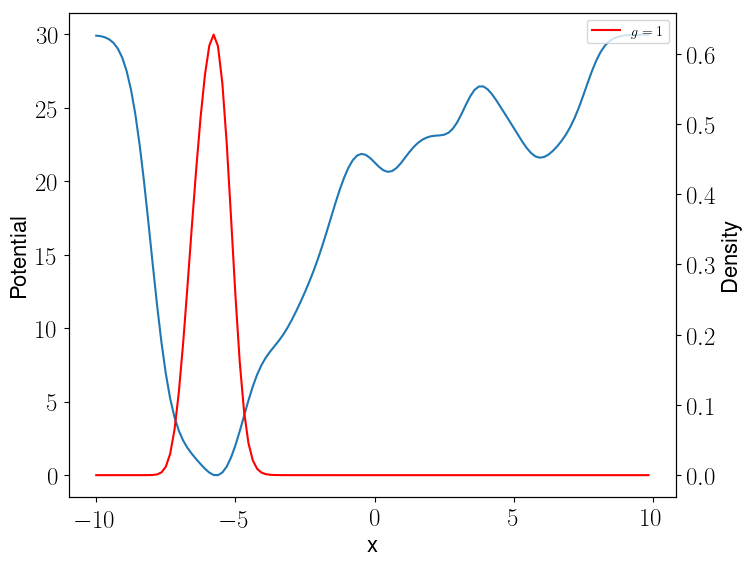
\includegraphics[width=\linewidth]{potvsdensity-random}
    \end{subfigure}
    \begin{subfigure}[t]{0.45\textwidth}
        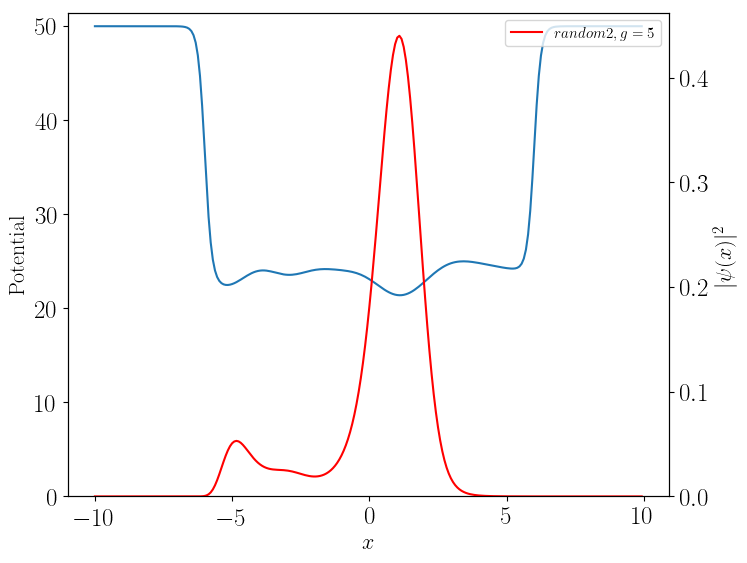
\includegraphics[width=\linewidth]{potvsdensity-random2}
    \end{subfigure}
    \begin{subfigure}[t]{0.45\textwidth}
        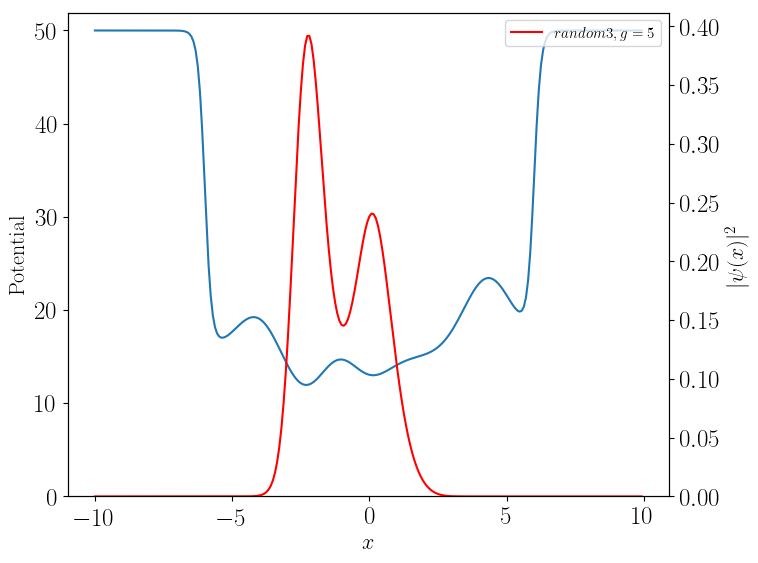
\includegraphics[width=\linewidth]{potvsdensity-random3}
    \end{subfigure}
\caption{Potentials and Corresponding Ground State Densities}
\label{fig:random3_before_after}
\end{figure}


%\subsubsection{Boundaries. (Table)}
%\subsubsection{Convergence (detailed in APPENDIX)}

\section{Machine Learning}
\label{sec:machine_learning}

Our aim is to show that the machine learning methods can be used to bypass GPE equation and physical features of the BEC can be predicted within high accuracy. To do that, we implemented a special type of artificial neural network called convolutional neural network (CNN). It is developed to handle data which have grid-like topology \cite{goodfellow2016deep} such as an image. Its strength occurs at when the subject has geometrical translation symmetry for instance the shape of a harmonic potential. In this section, we briefly introduce notions and mechanisms used in machine learning such as neuron, gradient descent etc. After that, we describe how these are used in our study.  

An artificial neural network is made of layers and these layers contain simple units called neurons. These neurons were inspired by the neurons in the human brain. A neuron takes one or more input and generates an output. To do this, it uses its internal variables which are called weights and biases. In general, the number of weights in a neuron is equal to the size of the input and there is one bias value. There is no restriction on the range of weights and biases except computational, they can even take on complex values \cite{zimmermann2011comparison}. Input output relation of a neuron can be described in the following way; if we represent the input of the neuron by $\boldsymbol{x} = [x_1, x_2, x_3, ..., x_n]$ and the function $f$ that describes behavior of the neuron can be written as, 

\begin{equation}
\label{eq:NU_neuron}
f(\boldsymbol{x}, \boldsymbol{\omega}, b) = \sum\limits_{i = 1}^n \omega_i x_i + b
\end{equation}

\noindent Here, $\omega_i$ are the weights and $b$ is the bias. A layer of a network involves neurons that implement with this function. In our example, $x_n$ inputs represent the potential expression respect to the position \footnote{We are using CNN with two channels; thus; the other channel is interaction parameter.} or represents density in the case of inverse problem. The range of the function $f$ is infinite and it can be used directly. However, there are various ways to interpret result of the function $f$. The most primitive version of interpretation is sending the result of $f$ as an argument to unit step function to generate 0 (False) or 1 (True). In this case, 

\begin{equation}
\label{eq:NU_step_function}
a(f) = u_1(f(\boldsymbol{x}, \boldsymbol{\omega}, b))
\end{equation}

\noindent where $a$ is called as the activation function of the neuron and it is a unit step function in this case. However, the usage of the step function introduces discontinuity and does not allow to use differential methods to calculate behavior of the neurons when a small change in weights or biases is applied. To handle this problem there are different activation functions. 
One of the most common activation function is sigmoid function denoted by $\sigma$ which is continuous version of the step function and it is defined as,

\begin{equation}
\label{eq:NU_sigma_function}
\sigma(f) = \frac{1}{1 + e^{-f}}
\end{equation}

\noindent If a neuron defined in this way such that its output given by Eq.~\eqref{eq:NU_sigma_function}, then it is called a sigmoid neuron. In the former case which is the step function, the neuron is called as perceptron. 

If we denote $j^{th}$ neuron in the $l^{th}$ layer with $f_j^l$, and the weight from $k^{th}$ neuron in the $(l-1)^{th}$ layer to the $j^{th}$ neuron in the layer $l^{th}$ with $\omega_{jk}^l$, finally the bias of the $j^{th}$ neuron in the $l^{th}$ layer with ${b_j^l}$, then, the output of the $j^{th}$ neuron in the $l^{th}$ layer will be;

\begin{equation}
\label{eq:NU_neuron_connection}
f_j^{l}(\sigma(f_k^{l-1}), \boldsymbol{\omega}, b) = \sum\limits_{k=1}^{n} \omega_{jk}^{l}\sigma(f_k^{l-1}) + b_j^l
\end{equation}

\noindent and the activation of the output can be written as;

\begin{equation}
\sigma(f_j^{l}(\sigma(f_k^{l-1}), \boldsymbol{\omega}, b)
\end{equation}


\noindent Here we use sigmoid function as activation function but it can be any suitable activation function such as hyperbolic tangent $\tanh(f)$ or Rectified Linear Unit (ReLU).

Connection complexity of the neurons may vary. Output of each neuron in one layer can be input of every neuron in next layer. Such networks are called Fully Connected Networks (FCN) or multilayer perceptrons (MLP). If the result of one layer is directly sent to the next layer without any circulation or feedback, then the network is called as Feed Forward Network \cite{nielsen2015neural}.

We are going to change these weights and biases in such a way that the difference between output generated by network and real value of the corresponding quantity will be minimized. To do that, we are going to use a proxy relation between output and real value which is called as Cost Function \cite{nielsen2015neural}. There are different kind of cost functions such as quadratic cost function, cross entropy cost function etc. We are going to use quadratic cost function also called as mean squared error to show the general mechanism and to introduce few notions that directly effects the behavior of the network. 


The quadratic cost function is defined as;

\begin{equation}
\label{eq:NT_Quadratic}
C(\omega, b) = \frac{1}{2n} \sum\limits_{x} || \boldsymbol{y} - a(f_L(\boldsymbol{x})) ||{^2} 
\end{equation}

\noindent where $n$, $\omega$, $b$ are number of examples in the training set, weights and biases, respectively. The subscript $L$ indicates the last layer which is the output, so $f_L(\boldsymbol{x})$ output produced by network and $\boldsymbol{y}$ is real value of the quantity. To minimize $C$, we can take derivative of the function and can find extremum values, but this method is extremely costly because the total number of neurons in the network is enormous \cite{nielsen2015neural}. This problem can be overcame by an iterative algorithm called Gradient Descent. Since $C$ is also a scalar field the algorithm tries to determine a direction which points to the decrement and moves in that direction with small steps. In each iteration, algorithm repeats itself to reach minimum value. 

A small displacement in arbitrary direction which corresponds to a small change in weight or bias or both can be written as;
\begin{equation}
\label{eq:NT_Quadratic_min}
\Delta{C} = \frac{\partial{C}}{\partial{\omega}}\Delta{\omega} + \frac{\partial{C}}{\partial{b}}\Delta{b}
\end{equation}

\noindent This expression gives information about what happens when small displacement is made. In order to the determine direction of decrement we can rewrite this expression in terms of the gradient since it points to direction of maximum rate of increase. We can define gradient operator as;

\begin{equation}
\label{eq:gradient}
\boldsymbol{\nabla}{C} = \left(\frac{\partial{C}}{\partial{\omega}},\frac{\partial{C}}{\partial{b}} \right)^T
\end{equation}

\noindent In this case, Eq.~\eqref{eq:NT_Quadratic_min} can be written as;

\begin{equation}
\label{eq:NT_Quadratic_min_gradient_form}
\Delta{C} = \boldsymbol{\nabla}{C} \cdot \Delta \boldsymbol{l}
\end{equation}

\noindent where $\boldsymbol{l} = (\omega, b)^T$. We want to minimize the cost function, thus; in each iteration value of the $C$ must be smaller than the previous one which means that $\Delta{C}$ must be smaller than zero. Therefore, the direction of displacement must be in the opposite direction of the gradient. Rather than calculating the opposite direction for each iteration we can define $\Delta{\boldsymbol{l}}$ in such a way so that it always points to opposite direction of the gradient.

\begin{equation}
\label{eq:NT_learning_rate}
\Delta{\boldsymbol{l}} = -\eta\boldsymbol{\nabla}C
\end{equation}

\noindent In this case, Eq.~\eqref{eq:NT_Quadratic_min_gradient_form} becomes;

\begin{equation}
\label{eq:NT_Displacement}
\Delta{C} = -\eta ||\boldsymbol{\nabla}{C}||^2
\end{equation}

\noindent where $\eta$ is positive definite number and it is called the learning rate. Since it is guaranteed that $||\boldsymbol{\nabla}{C}||^2 \geq 0$, therefore; $\Delta{C} \leq 0$. In this situation, learning rate is the step size in each iteration. From Eq.~\eqref{eq:NT_Displacement} it is intuitive that $\eta$ can not be a large number because in such a case, the algorithm can miss the minimum point. This situation also brings up the subject that gradient descent does not give guarantee to find the minimum point.

Gradient Descent algorithm has an statistical version called Stochastic Gradient Descent to increase the speed of training process. It is assumed that gradient of  $m$ randomly selected examples in the dataset is nearly equal to gradient of the whole dataset and it can be expressed as;

\begin{equation}
\label{eq:NT_Stochastic}
\frac{1}{m} \sum\limits_{k = 1}^{m} \nabla{C_{X_j}} \approx \frac{1}{n}\sum\limits_{x = 1}^{n} \nabla{C_{x}} = \nabla{C}
\end{equation}

\noindent where $\nabla{C_x}$ is the gradient of a single training input and $m$ is also called as mini-batch size.

It is worth noting that approaching a minimum value is proportional to the number of iterations which equals to number of examples in the dataset, therefore; it is a corollary that there can be two situations\footnote{The third case is that algorithm may diverge but we ignore this situation here.}. First, the algorithm cannot reach the minimum point due to lack of training examples, and secondly, the algorithm reaches a global or local minimum point and starts to oscillate around it \cite{zeiler2012adadelta}. There are mechanisms to prevent such cases and other optimization problems like direction sensitivity and they are called as adaptive learning rate. In our network we used an algorithm called Adam \cite{kingma2014adam} provided by the framework we used.  

The final step in the gradient descent is updating the weights and biases. We use Eq.~\eqref{eq:NT_Displacement} to perform this task. If we combine Eq.~\eqref{eq:NT_Displacement} with Eq.~\eqref{eq:NT_Stochastic} and write it in open form, the expression to update the weight and bias can be written as;

\begin{equation}
\label{eq:NT_weight_bias_update}
\begin{split}
& \omega^{\prime} = \omega - \frac{\eta}{m} \sum\limits_{j = 1}^{m} \frac{\partial{C_{X_j}}}{\partial{\omega}} \\
& b^{\prime} = b- \frac{\eta}{m} \sum\limits_{j = 1}^{m} \frac{\partial{C_{X_j}}}{\partial{b}}
\end{split}
\end{equation}

\noindent Numerical calculation of the partial derivatives in the equation is one of the costliest computational operation in the training process. To reduce computational cost, there is a well known algorithm called backpropagation \cite{goodfellow2016deep}. We use the framework we used it provides similar mechanism called automatic differentiation. 

\subsection{Network Architecture and Hyperparameters}

The CNN takes potential and interaction parameter as input and produce ground state energy as output. The network has six layers plus three 2D max-pooling layers with kernel size of two between convolution layers.. The first three of them are 1D convolution layers and the last three involving output layer are fully connected layers. Input layer has two channels, one for potential and one for interaction parameter. Output layer is involves only one neuron that represents energy value. The properties of the layers are given in the Table~\ref{tb:conv_layers} and~\ref{tb:fully_layers}.

\begin{table}[H]
    \centering
    \caption{Convolution Layers}
    \label{tb:conv_layers}
    \begin{tabular}{|l|l|l|l|l|} \hline
    \textbf{Layer}        & \textbf{In Channel} & \textbf{Out Channel}   & \textbf{Kernel Size}  \\ \hline
    Input                 & 2                   & 10                     & 2                     \\ \hline
    2\textsuperscript{nd} & 5                   & 20                     & 2                     \\ \hline
    3\textsuperscript{th} & 10                  & 20                     & 2                     \\ \hline
    \end{tabular}
\end{table}

\begin{table}[H]
    \centering
    \caption{Fully Connected Layers}
    \label{tb:fully_layers}
    \begin{tabular}{|l|l|l|l|l|} \hline
    \textbf{Layer}        & \textbf{Input}      & \textbf{Output}    \\ \hline
    4\textsuperscript{th} & 310                 & 100                \\ \hline
    5\textsuperscript{th} & 100                 & 20                 \\ \hline
    Output                & 20                  & 1                  \\ \hline
    \end{tabular}
\end{table}

We use ReLU as activation function and it is applied at each forward but no operation is applied to the output neuron. Here we give the hyperparameters of the network in the following table.

\begin{table}[H]
    \centering
    \caption{Hyperparameters}
    \label{tb:hyperparams}
    \begin{tabular}{|l|l|} \hline
    \textbf{Hyperparameter}  & \textbf{Size}  \\ \hline  
    Batch Size               & 50             \\ \hline
    Number of Epochs         & 100            \\ \hline
    Learning Rate $\eta$     & 0.003          \\ \hline
    \end{tabular}
\end{table}


\subsection{Dataset and Dataset Generation}

An element of a dataset has three components; the ground state energy of the system, an array containing potential respect to the position and interaction parameter. The interaction parameter is also included as an array same size with the potential to the dataset to make the input homogenous by increasing the channel number of the CNN. The interaction parameter can be introduced to the network with more sophisticated method to reduce computational cost but since we are working on 1D, the expense of not using such a method is relatively small.

The array containing potential is generated by one of the methods given in the section \ref{sec:potential_generation} and the interaction parameter is selected from a set of uniformly distributed numbers between 0 and 30. The energy values are obtained by the numeric solution framework. The total length of the dataset is 50000 for each potential type and 45000 of them are used as training dataset and 5000 of them as test dataset. 

\graphicspath{{"../figs/dataresults/"}}
\begin{figure}[H]
    \centering
    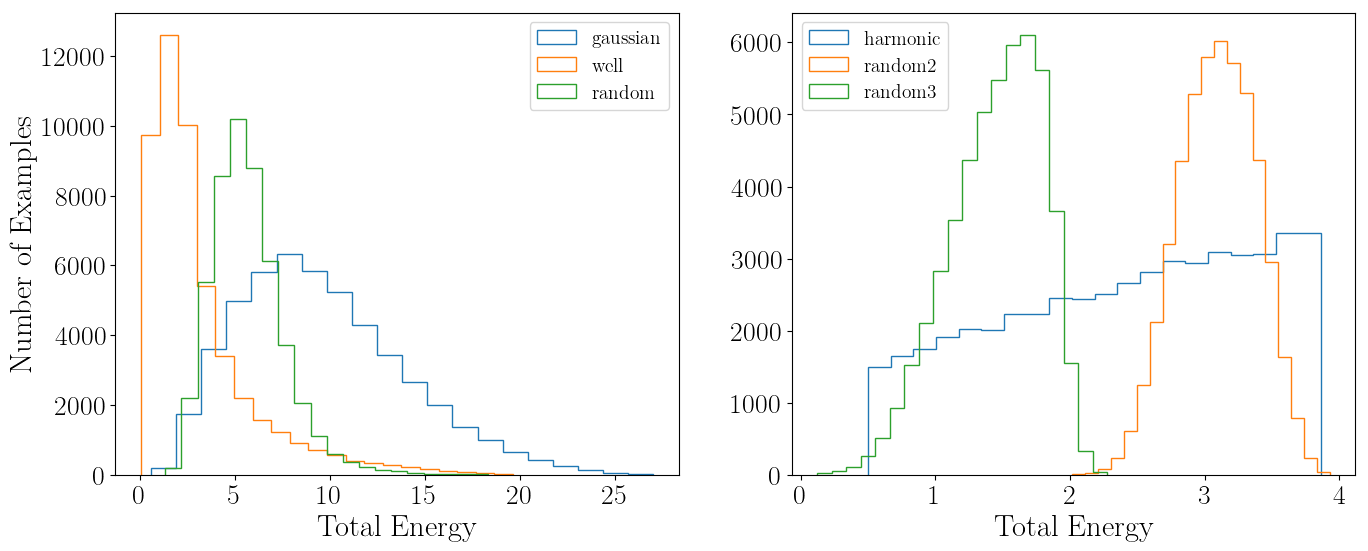
\includegraphics[width=\linewidth]{energydist}
\caption{The energy distribution of the random potentials are similar but it is clear that the random potential generation method directly affects the energy spectrum. There is a shift between energy spectrum of the random2 and random3. The random's spectrum is completely different and contains both random2's and random3's.}
\label{fig:energy_dist}
\end{figure}

Here in Fig.~\ref{fig:energy_dist} we give energy distribution histogram of the dataset. Because of non-linearity, the energy distribution is not uniform. The closest one is harmonic potential.


\subsection{Machine Learning Framework}

We used Pytorch Framework \cite{paszke2017automatic} to build our neural networks. It allows the client codes to work on both CPU and GPU via its internal python object called Tensor. If any CUDA supported GPU is available then Pytorch can use GPU without any change in the code. Machine Learning code has three main parts, first one is dataloaders; it reads train and test data from corresponding file and generates tensor dataset object. In this part, manipulation on dataset can be applied such as normalization, shuffling etc. Second part is implementation of the network. Architecture of the network is represented with a python class inherited from Pytorch's base class for networks called Module. This class also includes a forward method which is responsible for how data will be sent to the next layer. The last part is training and testing. In the training part, the network is iterated with training dataset and loss (result of cost function) is calculated at the end of each iteration. After that, weights and bias are updated accordingly by framework.

\subsection{Training Results}
\label{sec:training_results}

In the training process, we investigate three different scenarios. The first one is training and testing neural network with same potential type. The second one is cross test such that the type of potential in training and test process is different. The third and the last one is mixing the all potential types into one and generating new dataset by randomly choosing \textbf{N} elements.

\graphicspath{{"../figs/training/"}}
\begin{figure}[H]
    \centering
    \begin{subfigure}[t]{0.49\textwidth}
        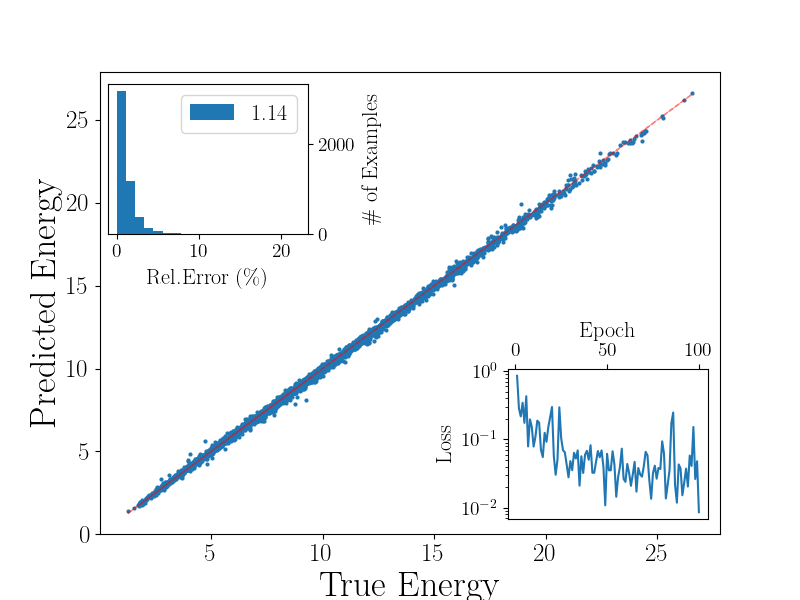
\includegraphics[width=\linewidth]{gaussian}
    \caption{Double Inv. Gaussian}
    \end{subfigure}
    \begin{subfigure}[t]{0.49\textwidth}
        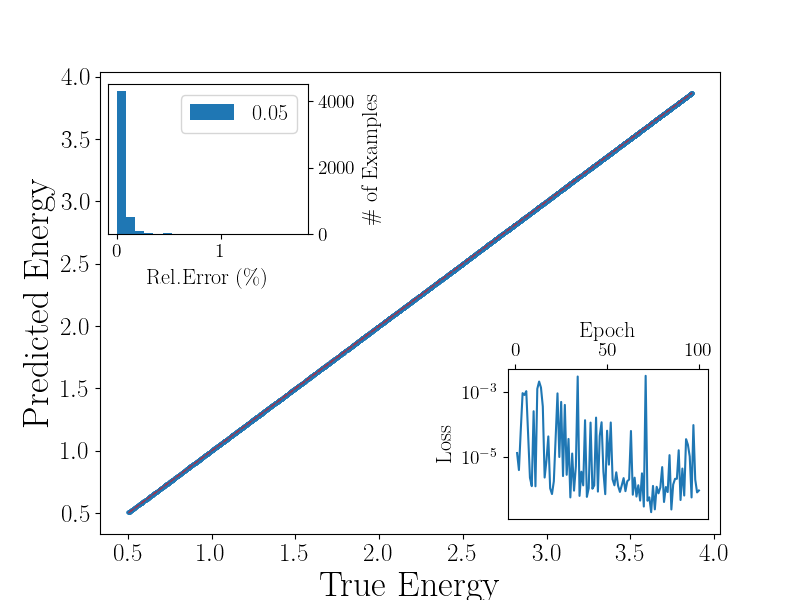
\includegraphics[width=\linewidth]{harmonic}
    \caption{Harmonic}
    \end{subfigure}
    \begin{subfigure}[t]{0.49\textwidth}
        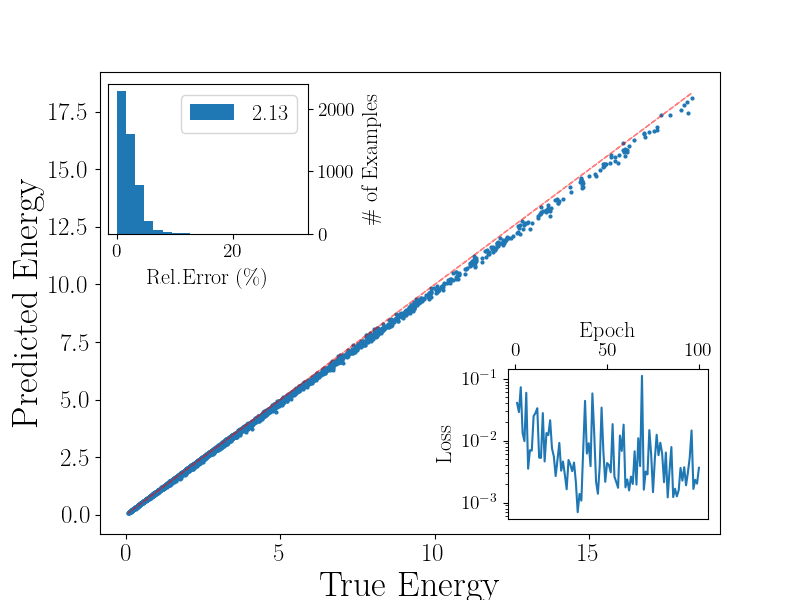
\includegraphics[width=\linewidth]{well}
        \caption{Infinite Well}
    \end{subfigure}
    \begin{subfigure}[t]{0.49\textwidth}
        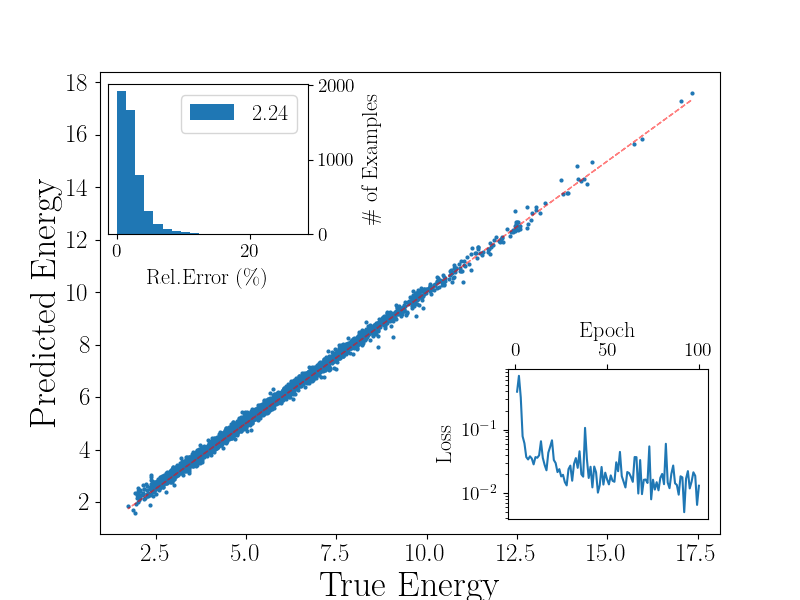
\includegraphics[width=\linewidth]{random}
        \caption{Random Type 1}
    \end{subfigure}
    \begin{subfigure}[t]{0.49\textwidth}
        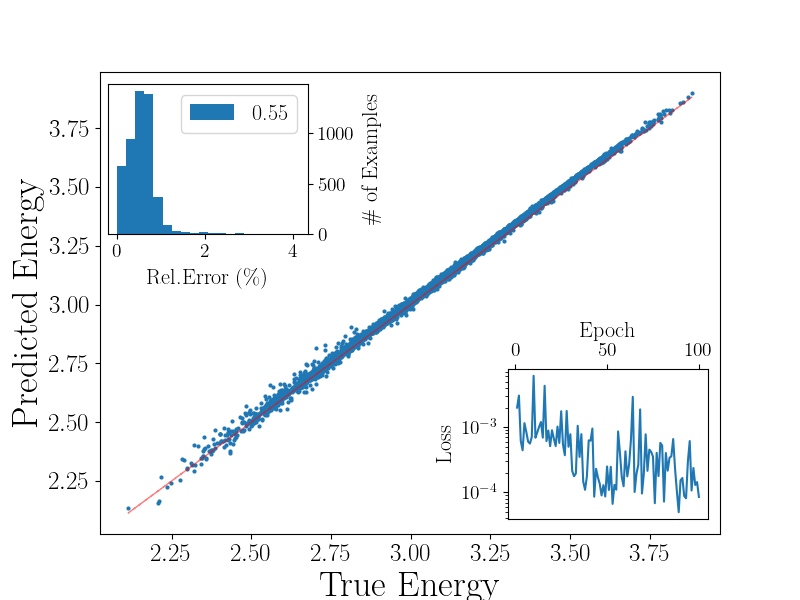
\includegraphics[width=\linewidth]{random2}
        \caption{Random Type 2}
    \end{subfigure}
    \begin{subfigure}[t]{0.49\textwidth}
        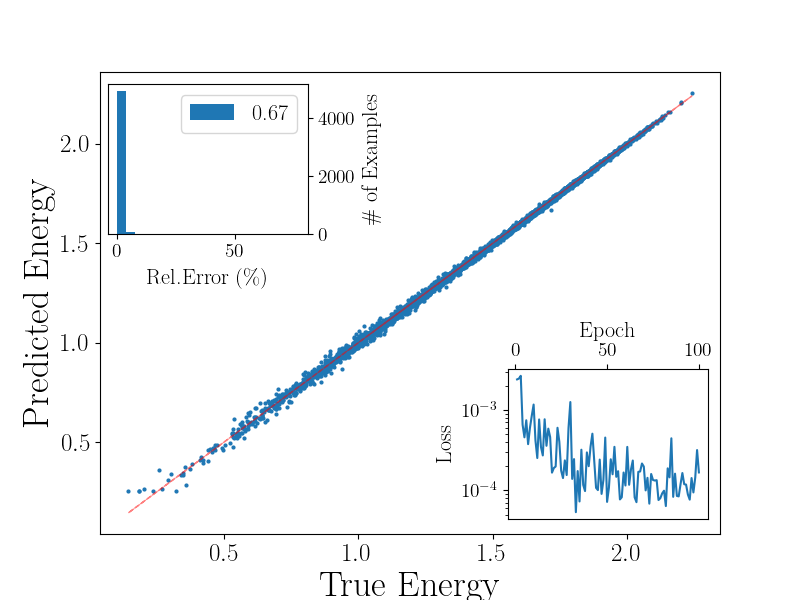
\includegraphics[width=\linewidth]{random3}
        \caption{Random Type 3}
    \end{subfigure}
\caption{Here training and test potential types are the same and they are labeled. The upper left insets are relative error histograms and the bottom right figures show loss per epoch. The legends of the histograms represents the mean of the relative errors.}
\label{fig:training_results}
\end{figure}

The energy distribution given in Fig.~\ref{fig:energy_dist} shows itself in results. Except harmonic potential, the number of examples in lower or higher energies are rare compared to the mean. The mean of relative errors are lower than $3\%$ and the smallest case is harmonic potential with $0.05\%$

The second case's results are not satisfactory. The mean of relative errors are up to $100\%$ and more. Here we give the most successful result in the following figure. 

\graphicspath{{"../figs/training/cross-training/"}}
\begin{figure}[H]
    \centering
    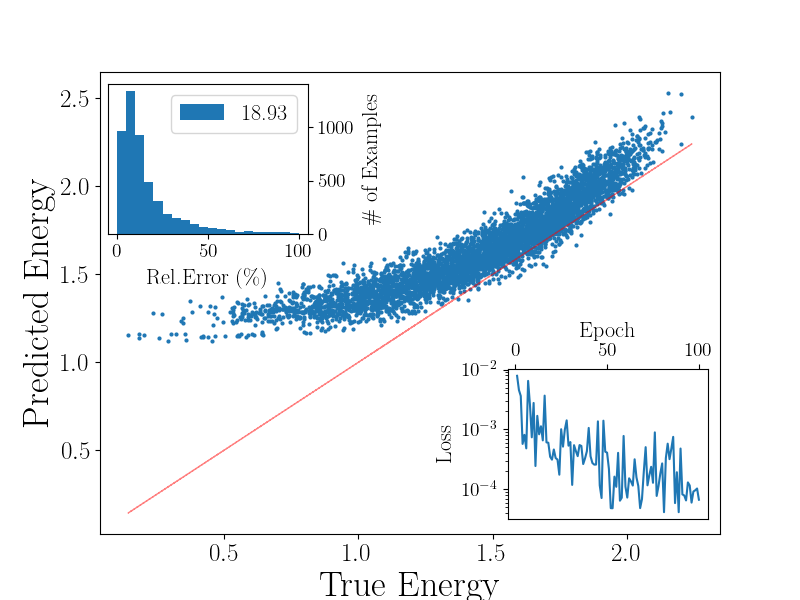
\includegraphics[width=0.6\linewidth]{random2-random3}
\caption{In this test, the network is trained with Random Type 2 and tested with Random Type 3.}
\label{fig:cross_training_results}
\end{figure}

As indicated before, energy spectrum directly effects the results. The spectrum intersection of random potentials given in the Fig.~\ref{fig:cross_training_results} is very small which means the network nearly does not see any example that looks like tested random potential.


\graphicspath{{"../figs/training/combined/"}}
\begin{figure}[H]
    \centering
    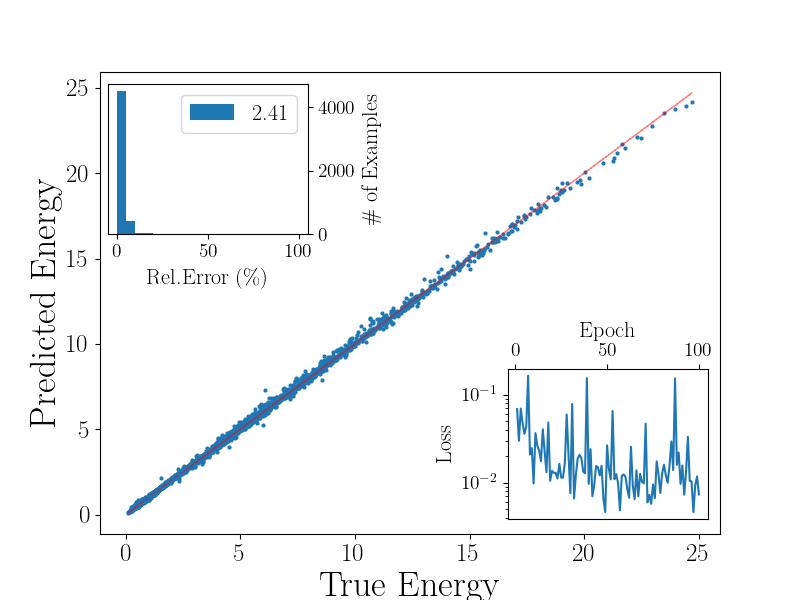
\includegraphics[width=0.6\linewidth]{main}
\caption{In this test, the network see all types of potentials.}
\label{fig:comb_training_results}
\end{figure}

Here we give last scenario in Fig~\ref{fig:comb_training_results}. The network is trained with 100000 examples chosen randomly from whole dataset.  



\section{Inverse Problem}

In the inverse problem, we train the neural network with potential and density to predict interaction parameter of the system. The neural network used in this scenario is identical to the previous one. The only change is what input and output represents. In this time, input channels represents potential and density, the output channel represents the interaction parameter. The dataset of the inverse problem is made by concatenating all previous datasets and selecting one hundred thousand random elements. 

\graphicspath{{"../figs/training/interaction/"}}
\begin{figure}[H]
    \centering
    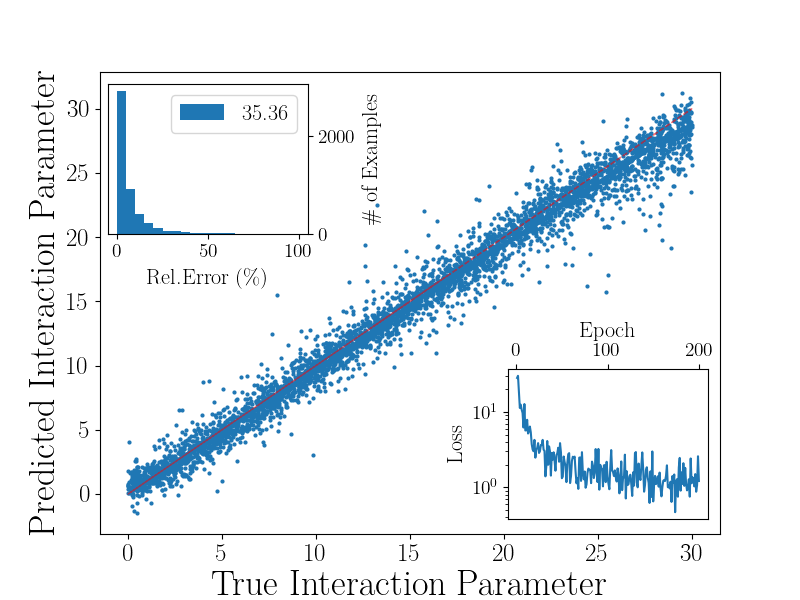
\includegraphics[width=0.6\linewidth]{gaussian-inter}
\caption{Results of inverse problem, predicting interaction parameter. The number of epochs is increased to the 200. }
\label{fig:inverse_results}
\end{figure}

\clearpage
\section{Conclusion and Discussion}

In this study, we applied machine learning technique to the non-linear Schr\"{o}dinger equation also known as Gross-Pitaevskii equation. In section~\ref{sec:training_results} it is shown that an artificial neural network can predict ground state energy of a Bose-Einstein condensate that involves repulsive interaction with $2.24\%$ mean relative error. However, this situation only holds when the training and test examples are same type potentials. In Fig.~\ref{fig:cross_training_results} it is obvious that the neural network is not able to make prediction with high precision in the case of cross training. This situation brings another subject which is the effect of the random potential generation process. We implemented three different random potential generators to investigate this effect. In all cross training scenarios the neural network is not able to make prediction with an acceptable precision. We suspect from two reasons why such poor predictions occurred. The first one is energy spectrum; the three of the random potential solutions nearly does not share a common energy spectrum. The second one is energy distribution; the neural network does not see uniformly distributed examples and because of this reason it becomes biased. In the third scenario, the network showed the same success as in the first one. The relative mean error is $2.41\%$ but again the number of examples in the higher energies are low.  

In the inverse problem, we used the identical network to predict interaction parameter. The network is supplied with potential and density as input and the mean relative error of the predictions is $35.36\%$. To overcome this precision problem, the total number of layers can be increased since we used identical networks but density array contains much more information than interaction parameter. The neural network's degree of freedom must be enough to handle this amount of information. 

\subsection{Future Work}

The cross training results can be improved by fixing the problems we mentioned. To do that, there are two options; one of them is changing interaction parameter's range and distribution such a way so that the energy spectrum and distribution will be in desired form. The second way which is generalized version of previous one is also manipulating random potential generation process without biasing randomness. The second option is an entire new problem; therefore; we are going to follow the first way. To determine interaction parameter's range and distribution, we are going to use variational method for lower values and Thomas-Fermi approximation for higher values.


\clearpage

\clearpage
\bibliographystyle{ieeetr}
\bibliography{references}

\end{document}

%
%
%\appendix
%\section{APPENDIX A}
%\label{ap:scale}
%
%Obtaining harmonic trap potential scaling from Eq.~\eqref{eq:GPE_dimensionless}
%
%\begin{equation}
%\label{eq:GPESCALE_harmonic_potential_transform}
%    V(x) \rightarrow V(\widetilde{x}) \rightarrow \widetilde{V}(\widetilde{x})
%\end{equation}
%
%\begin{equation}
%\label{eq:GPESCALE_dimensionless_harmonic_potential}
%    \widetilde{V}(x) \equiv \frac{V(x)}{\gamma E_0}
%\end{equation}
%
%\begin{equation}
%\label{eq:GPESCALE_dimensionless_length}
%    \widetilde{x} \equiv \frac{x}{\beta L} 
%\end{equation}
%
%\begin{equation}
%\label{eq:GPESCALE_harmonic_potential}
%    V(x) = \frac{1}{2}m\omega^2 (x-z_0)^2
%\end{equation}
%
%\begin{equation}
%\label{eq:GPESCALE_harmonic_length_transform}
%    V(\widetilde{x}) = \frac{1}{2}m\omega^2 \beta^2 L^2 (\widetilde{x}-\widetilde{z_0})^2
%\end{equation}
%
%\begin{equation}
%\label{eq:GPESCALE_harmonic_energy_transform}
%    \widetilde{V}(\widetilde{x}) = \frac{1}{2} m\omega^2 \frac{\beta^2 L^2}{\gamma E_0} (\widetilde%{x}-\widetilde{z_0})^2  
%\end{equation}
%
%\noindent The coefficient of this equation must be dimensionless, therefore;
%
%\begin{equation}
%\label{eq:GPESCALE_harmonic_coeff}
%    \frac{1}{2} m\omega^2 \frac{\beta^2 L^2}{\gamma E_0} = C
%\end{equation}
%
%\noindent Where $C$ is a positive constant. We know that $E_0 = \frac{\hbar^2}{2m}$ and the %definition of $\alpha$ is given as,
%
%\begin{equation}
%\label{eq:GPESCALE_alpha}
%    \frac{\hbar^2}{2m\gamma E_0} \frac{1}{\beta^2 L^2} = \alpha
%\end{equation}
%thus;
%
%\begin{equation}
%\label{eq:GPESCALE_gamma}
%     \frac{1}{\gamma} = \alpha \beta^2 L^2
%\end{equation}
%
%\noindent if we plug Eq.~\eqref{eq:GPESCALE_gamma} in to Eq.~\eqref{eq:GPESCALE_harmonic_coeff}, %then equation becomes,
%
%\begin{equation}
%\label{eq:GPESCALE_harmonic_coeff_2}
%    \frac{m^2\omega^2}{\hbar^2} \alpha \beta^4 L^4 = C 
%\end{equation} 
%
%\noindent In this case, $\alpha$ becomes
%
%$$ \alpha =  \frac{1}{2} \left(\frac{\hbar \omega}{\gamma E_0}\right)^2 $$
%
%\noindent Conventionally, $\alpha$ is set to $1/2$, therefore;
%
%$$ \hbar \omega = \gamma E_0 $$
%
%$$ \beta L = \sqrt{\frac{\hbar}{m\omega}} $$ 
%
%\noindent $ \beta L $ is generally defined as harmonic oscillator length $\ell$
%
%$$ \ell = \sqrt{\frac{\hbar}{m\omega}} $$ 
%
%$$ \widetilde{\mu} = \frac{\mu}{\hbar \omega} $$ 
%
%$$ \widetilde{g} = \frac{g}{\hbar \omega \ell} $$
%
%\noindent Finally, dimensionless GPE scaled for harmonic trapping potential can be written as,
%
%$$\widetilde{\mu} \widetilde{\psi} = -\frac{1}{2}\frac{d^2\widetilde{\psi}}{d\widetilde{x}^2} + %\frac{1}{2}\widetilde{x}^2\widetilde{\psi} + \widetilde{g}|\widetilde{\psi}|^2 \widetilde{\psi} $$
%

